\chapter{Demo}

In order to showcase the work we have done, we have also built a small web application capable of performing lyrics featurization and classification to define emotional patterns in a given playlist. Its home page is shown in figure \ref{fig:demo-home}.

\begin{figure}[H]
  \centering
  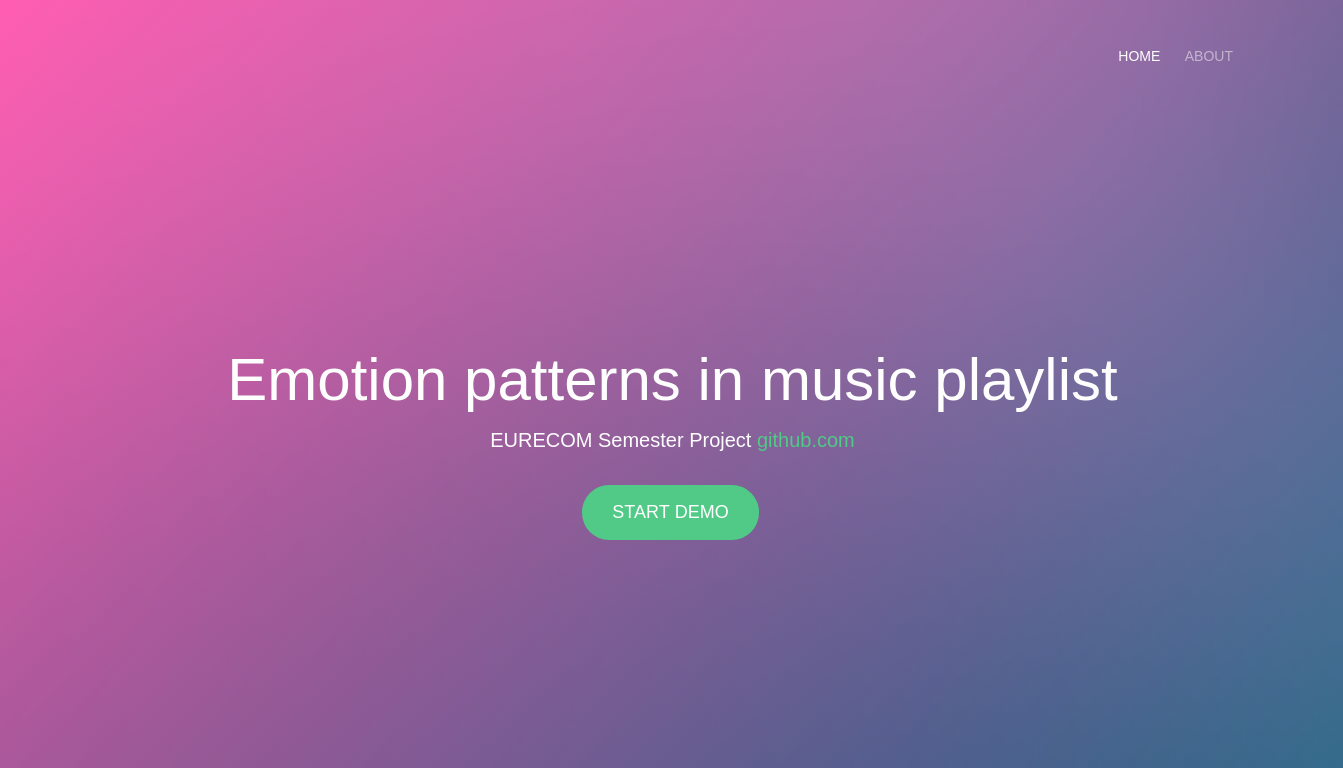
\includegraphics[width=1.0\textwidth]{./chapters/appendix1/images/home-page}
  \caption{Project demo home page}
  \label{fig:demo-home}
\end{figure}

Our demo is a web application, using the standard HTML, JavaScript and CSS tehcnologies and a few more libraries (jQuery\footnote{\url{https://jquery.com/}}, Bootstrap\footnote{\url{https://getbootstrap.com/}} and Plotly\footnote{\url{https://plot.ly/javascript/}}) for the front-end part. The back-end part, instead, was developed using Python and Flask\footnote{\url{http://flask.pocoo.org/}}.

The server has the only purpose of serving our static pages and to provide endpoints to perform lyrics classification.

From the home page, a user can either have a look at a description of the project by visiting the ``About'' page or he can starts the real demo by hitting the ``START DEMO'' button.

The playlists to classify are taken from Spotify, using their public REST API\footnote{\url{https://developer.spotify.com/documentation/web-api/}}. This is the reason why users are asked to login with their Spotify account if they want to be able to use the demo itself.

Once the user is logged in and he has the Spotify's URL of the playlist he wants to classify, he just has to hit the ``Classify Songs'' button (shown in figure \ref{fig:demo-form}) and wait for the termination of the operation. 

\begin{figure}[H]
  \centering
  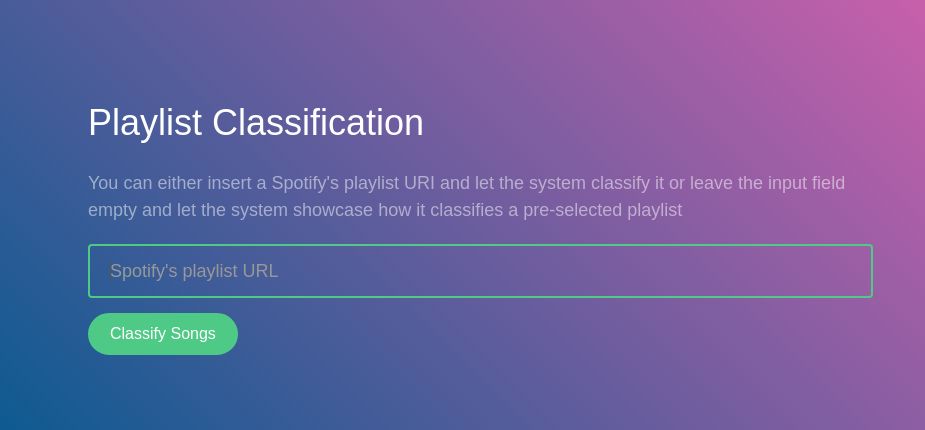
\includegraphics[width=1.0\textwidth]{./chapters/appendix1/images/demo-input}
  \caption{Playlist Classification Input Page}
  \label{fig:demo-form}
\end{figure}

When the user starts classifying a playlist, in the background, each song lyrics is downloaded, featurized and classified and a table will appear with the results of this operation. After that all songs in the playlist are classified, the user is able to finally classify also the playlist by hitting the button ``Classify Playlist'' (shown in figure \ref{fig:demo-playlist-classify}).

\begin{figure}[H]
  \centering
  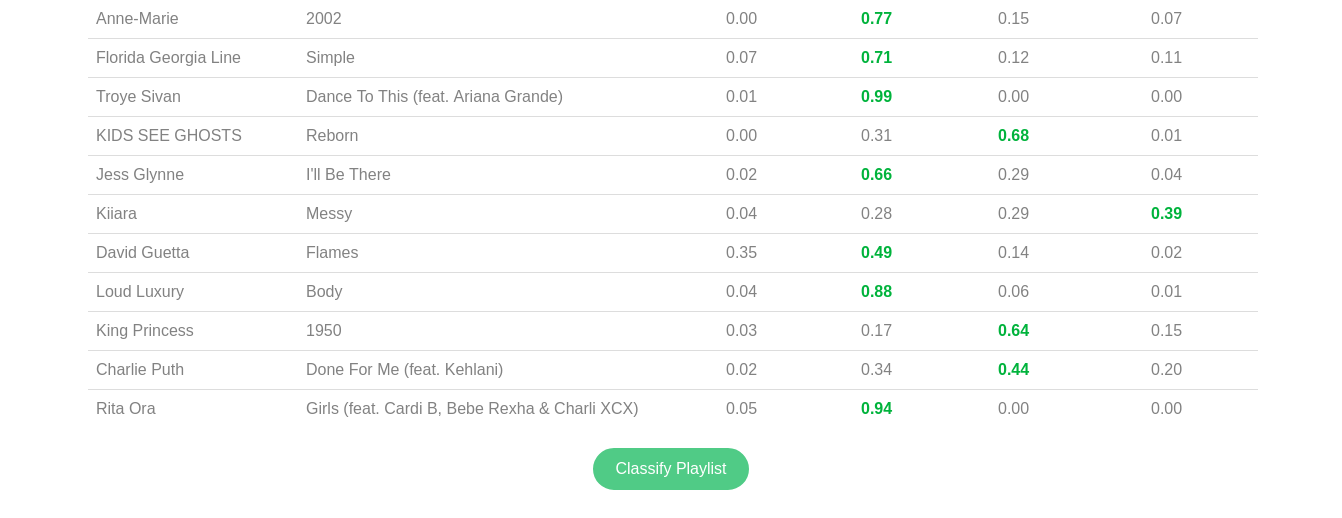
\includegraphics[width=1.1\textwidth]{./chapters/appendix1/images/demo-playlist-classify}
  \caption{Part of the results obtained when classifying a playlist}
  \label{fig:demo-playlist-classify}
\end{figure}

After the user has decided to classify the entire playlist, he will be shown with the score for each emotion assigned to the playlist and he will be able to see the emotional pattern which was found in it. An example of how those results would appear is shown in figure \ref{fig:demo-final-result}.

\begin{figure}
  \centering
  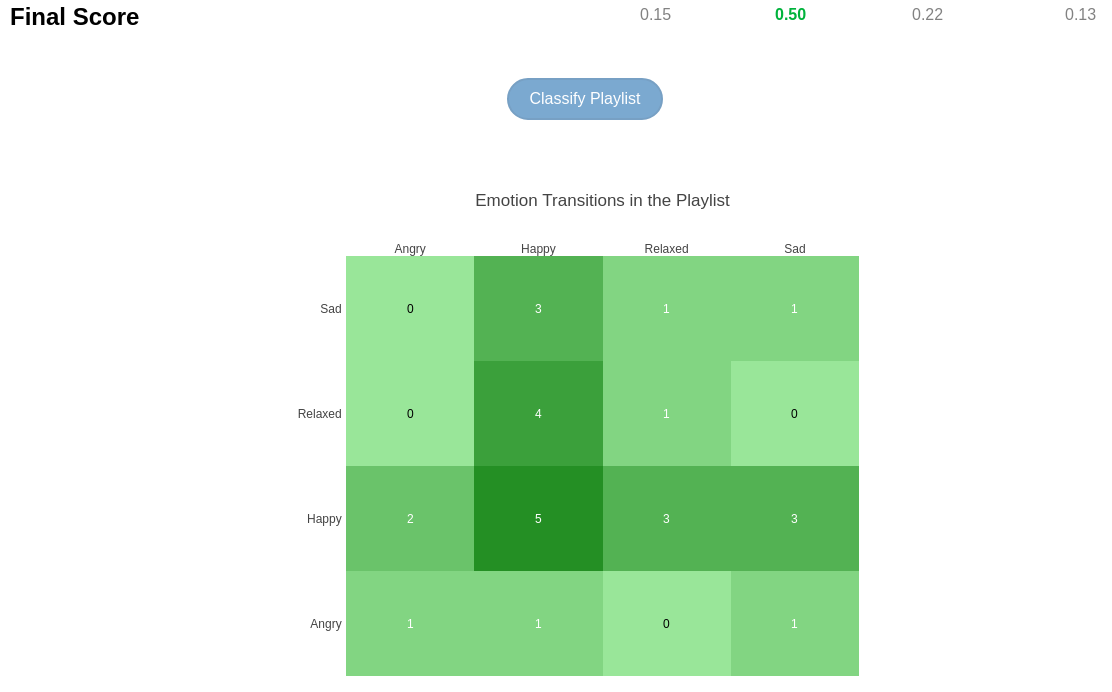
\includegraphics[width=1.0\textwidth]{./chapters/appendix1/images/demo-final-result}
  \caption{Part of the results obtained when classifying a playlist}
  \label{fig:demo-final-result}
\end{figure}

This web application was hosted on EURECOM's servers. It can be reached at \url{URL_HERE}.